% !TEX root = ../main.tex:532

\setCJKfamilyfont{hei}{SimHei}[Scale=0.9]
\setCJKfamilyfont{sun}{Source Han Serif SC Medium}[Scale=0.8]
\newcommand{\hei}{\CJKfamily{hei}\selectfont}
\newcommand{\sun}{\CJKfamily{sun}\selectfont}

\vspace*{1.5cm}

% 2025 :532
% \begin{picture}(400,60)(0,0)
% 	\put(10, 0){\includegraphics[width=200\unitlength]{cover/sjtubannerred.pdf}}
% 	\put(295,32){\fontsize{20.3}{1}\fontspec[]{Linux Libertine O}\color{black}ICPC World Finals Dhaka}
% 	\put(295, 6){\fontsize{23}{1}\fontspec[]{Linux Libertine O}\color{black}Standard Code Library}
% \end{picture}

\vspace*{1cm}
\begin{figure*}[h]
	\centering
	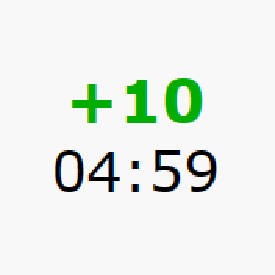
\includegraphics[width=180pt]{cover/logo.pdf}
\end{figure*}
\vspace*{0.75cm}
\centerline{{\fontsize{40}{1}{{\fontspec{Gill Sans Medium}Plenty of Penalty}}}}
\vspace*{3.5cm}
\begin{center}
{\LARGE
\begin{tabular}{cp{1in}c}
\rule{0pt}{16pt} \textbf{Coach} & & {\hei{教练}} \\
\midrule
\rule{0pt}{16pt} Can Wang & & {\sun 王灿} \\
\\\\
\rule{0pt}{16pt} \textbf{Contestant} & & {\hei{队员}} \\
\midrule
\rule{0pt}{16pt} Yulun Wu & & {\sun 吴与伦} \\
\rule{0pt}{16pt} Ruiyang Xu & & {\sun 徐锐扬} \\
\rule{0pt}{16pt} Hong Wan & & {\sun 万弘} \\
\end{tabular}
}
\end{center}

\vspace*{1cm}
\centerline{\large Compiled on \today}
\newpage